\section{Hausdorff Distance}  
Let $A$ and $B$ be sets in the plane. The \textit{directed Hausdorff distance} is: 
\begin{equation}\label{eqn:ContactGraphV3-1}
d\lr{A,B} = \sup_{a \in A} \inf_{b \in B} \left\vert\left\vert a-b \right\vert \right\vert
\end{equation}
$d\lr{A,B}$ finds the furthest point $a \in A$ from any point in $B$.  \textit{Hausdorff distance} is
\begin{equation}\label{eqn:ContactGraphV3-2}
D\lr{A,B} = \max \left\lbrace d\lr{A,B}, d\lr{B,A} \right\rbrace
\end{equation}

In Figure \ref{fig:HausdorffDistanceExample1.pdf}, we have two sets $X$ and $Y$ and illustrate $d(X,Y)$ and $d(Y,X)$.  
From this, it is possible to calculate the Hausdorff distance between $X$ and $Y$.

\begin{minipage}{\linewidth}
\begin{center}
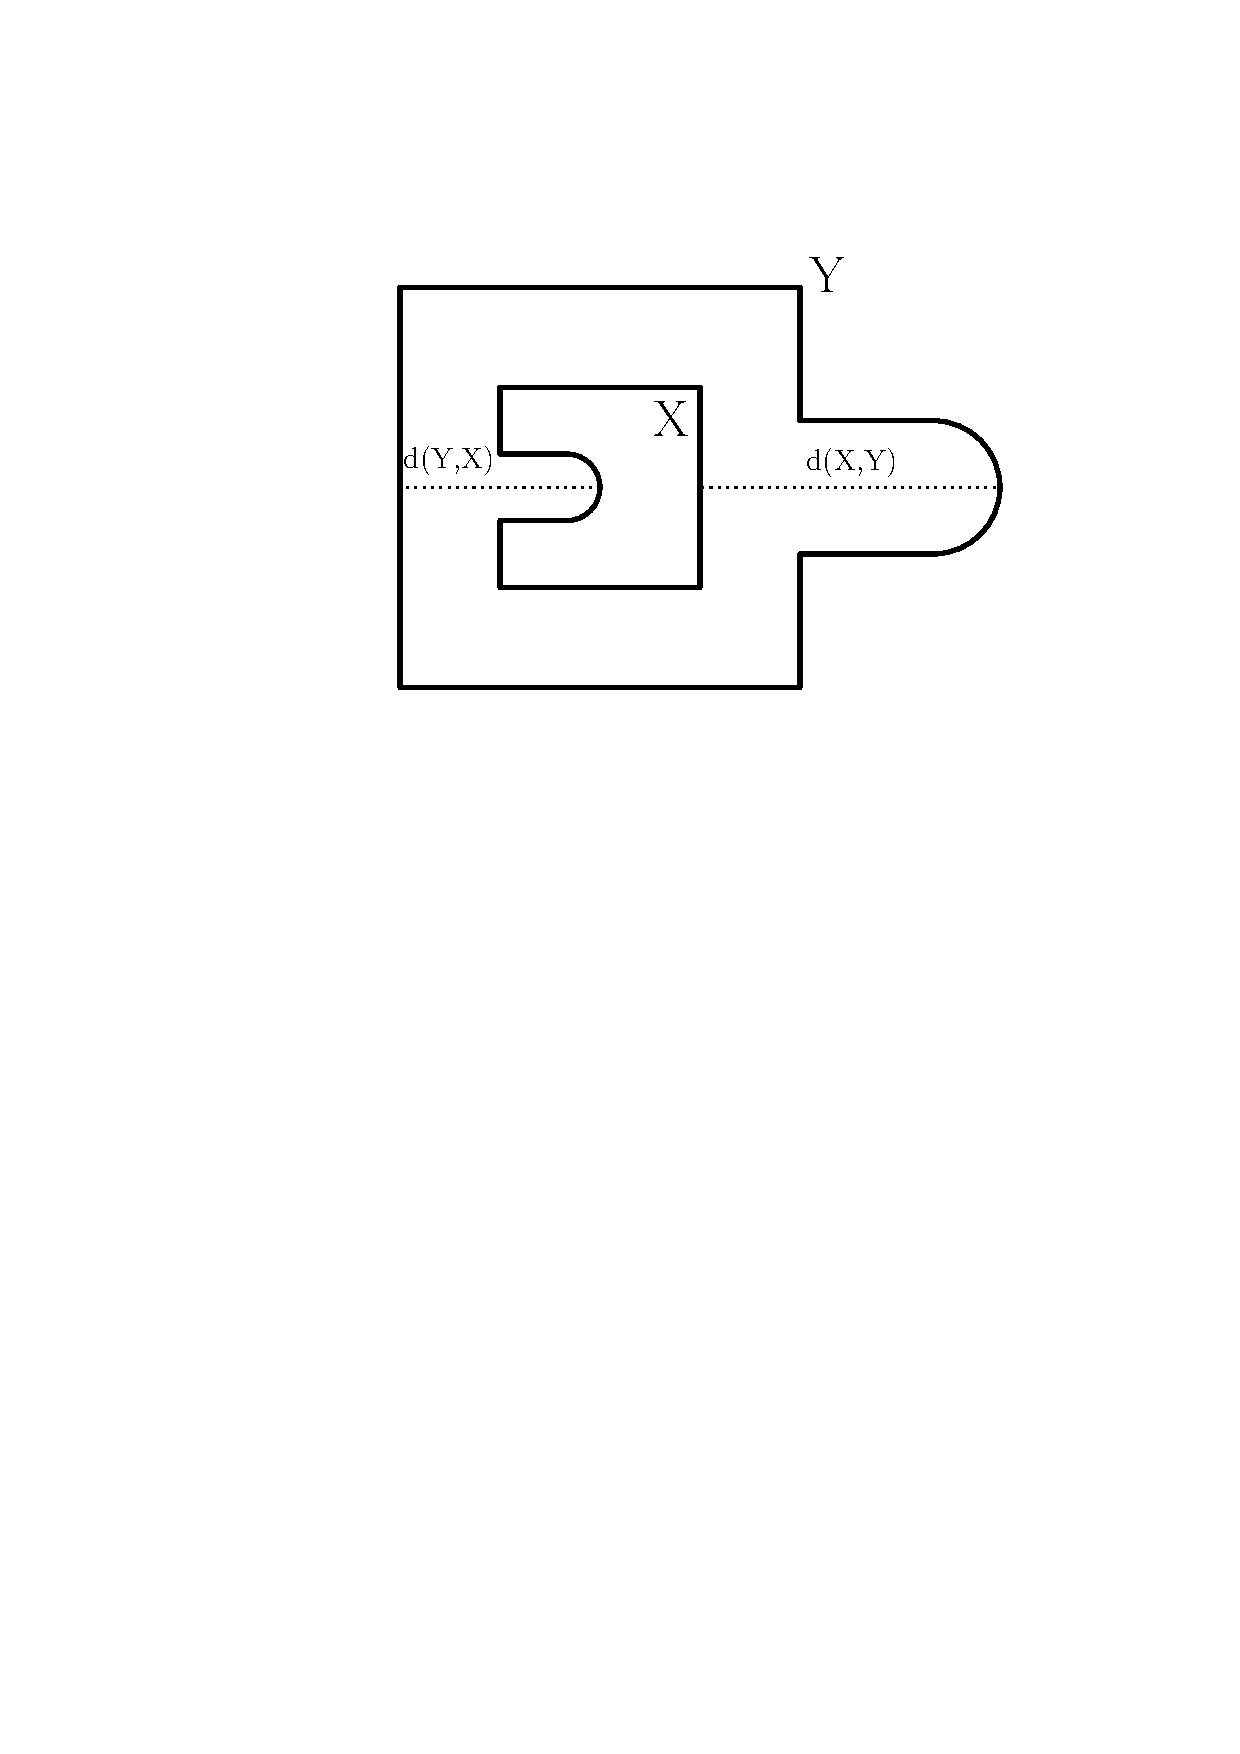
\includegraphics[width=.33\columnwidth]{graphics/HausdorffDistanceExample1.pdf}
\captionof{figure}{An illustrative example of $d(X,Y)$ and $d(Y,X)$ where $X$ is the inner curve, and $Y$ is the outer curve.}\label{fig:HausdorffDistanceExample1.pdf}
\end{center}
\end{minipage}

\paragraph{$\epsilon$-approximation}
The weighted graph, $G$, is an \textit{$\epsilon$-approximation} of a polygon $P$ if the Hausdorff distance between every realization of $G$ as a contact graph of disks and a congruent copy of $P$ is at most epsilon.  
A weighted graph $G$ is said to be a \textit{$\BigOh{f(x)}$-approximation} of a polygon P if there is a positive constant $M$ such that for all sufficiently large values of $x$ the Hausdorff distance between every realization such realization of $G$ as a contact graph of disks and a congruent copy of $P$ is at $M \cdot \vert f(x)\vert$. 
A weighted graph $G$ is said to be a \textit{stable} if it has the property that for every two such realizations of $G$, the distance between the centers of the corresponding disks is at most $\epsilon$ after a suitable rigid transformation.

Suppose we have a unit disk $U$ and we have a grid overlayed on the disk with side length $\delta$.  
Let $S_1(\delta)$ be the union of grid squares completely in the interior of $U$.  
Let $S_2(\delta)$ be the union of squares that intersect $U$.  
The Hausdorff distance of $U$ and $S_1(\delta)$ is at most $H\lr{S_1(\delta), U}\leq\sqrt{2}\delta$.  
Similarly, the Hausdorff distance of $U$ and $S_2(\delta)$ is at most $H\lr{S_2(\delta), U}\leq\sqrt{2}\delta$.
For any $\epsilon>0$, choose a $\delta$ such that $\sqrt{2}\delta \leq \epsilon$. Then the Hausdorff distance between $U$ and $S_1(\delta)$, $U$ and $S_2(\delta)$ is: 
$$
\begin{array}{rcl}
H\lr{S_1(\delta), U}&\leq&\sqrt{2}\delta\\
H\lr{S_2(\delta), U}&\leq&\sqrt{2}\delta
\end{array}
$$  
Similiaryly, the Hausdorff distance of $U$ and $S_2(\delta)$ is at most $H\lr{S_2(\delta), U}=\sqrt{2}\delta$.

\begin{lem}\label{lem:ch4IntroLemma}
For every $\epsilon > 0$ and $x>0$, there exists an ordered weighted tree $T_\epsilon$ and regular hexagon $h$ of side length $x$ such that:
\begin{enumerate}
\item Every realization $r$ of $T_\epsilon$ as an ordered disk contact graph where the radii of the disks equal the vertex weights, approximates the hexagon in the sense that:
$$H\lr{r\lr{T_\epsilon},h}=\epsilon$$
\item The number of nodes in $T_\epsilon$ and the weights are polynomial in $\epsilon$ and $x$.
\end{enumerate}
\end{lem} 

Lemma \ref{lem:ch4IntroLemma} is rather restrictive; it begs the question of whether it can be generalized. Some ways this lemma could be generalized are: (1) if all weights are equal, (2) order does not matter, and (3) if we relax the regular hexagon to any arbitrary polygon. 
